% Created 2020-10-08 Thu 15:23
% Intended LaTeX compiler: pdflatex
\documentclass[presentation]{beamer}
\usepackage[utf8]{inputenc}
\usepackage[T1]{fontenc}
\usepackage{graphicx}
\usepackage{grffile}
\usepackage{longtable}
\usepackage{wrapfig}
\usepackage{rotating}
\usepackage[normalem]{ulem}
\usepackage{amsmath}
\usepackage{textcomp}
\usepackage{amssymb}
\usepackage{capt-of}
\usepackage{hyperref}
\usetheme{UoB}
\author{Mark Blyth}
\date{}
\title{MatCont and PyDSTool}
\hypersetup{
 pdfauthor={Mark Blyth},
 pdftitle={MatCont and PyDSTool},
 pdfkeywords={},
 pdfsubject={},
 pdfcreator={Emacs 27.1 (Org mode 9.3)}, 
 pdflang={English}}
\begin{document}

\maketitle


\section{Slides}
\label{sec:orgcee6a65}
\begin{frame}[label={sec:org6d22fe2}]{Intro to MATCONT}
MATCONT is a MATLAB-based bifurcation analysis tool
\vfill
\begin{itemize}
\item GUI version (demo'd here), and command-line version
\end{itemize}
\vfill
\begin{itemize}
\item Both do the same thing; command-line is useful for big software projects, GUI version for standalone analyses
\end{itemize}
\vfill
\begin{itemize}
\item Fully integrated into MATLAB
\end{itemize}
\vfill
\begin{itemize}
\item More sleek interface than XPP, and less prone to crashing!
\end{itemize}
\end{frame}

\begin{frame}[label={sec:orge2f36b7}]{MATCONT vs XPP}
\begin{center}
\begin{tabular}{llll}
\hline
Feature & MatCont & XPPAUTO & PyDSTool\\
\hline
ODEs & y & y & y\\
PDEs (discretized) & n & y & n\\
DDEs & n & y & limited\\
SDEs & n & y & limited\\
DAEs & n & y & y\\
BVPs & n & y & n\\
Hybrid systems & n & limited & y\\
Main language & MATLAB & C & Python\\
Simulation tools & y & y & y\\
\hline
\end{tabular}
\end{center}
\end{frame}

\begin{frame}[label={sec:org197f943},plain]{MATCONT vs XPP}
\begin{center}
\begin{tabular}{lrlll}
\hline
Bifurcation Type & Codimension & MatCont & XPPAUTO & PyDSTool\\
\hline
Equilibrium & 0 & C & D,C & D,C\\
Limit cycle & 0 & C & C & C\\
Limit point & 1 & D,C & D,C & D,C\\
Hopf & 1 & D,C & D,C & D,C\\
Limit point of cycles & 1 & D,C & - & D\\
Neimark-Sacker & 1 & D,C & D,C & D,C\\
Period doubling & 1 & D & D,C & D,C\\
Homoclinic & 1 & C & C & -\\
Cusp & 2 & D & - & D\\
Bogdanov Takens & 2 & D & - & D\\
Zero-Hopf & 2 & D & - & D\\
Double Hopf & 2 & D & - & D\\
Generalised Hopf & 2 & D & - & D\\
Cusp point of cycles & 2 & D & - & -\\
Chenciner & 2 & D & - & -\\
Fold-Neimark-Sacker & 2 & D & - & -\\
Flip-Neimark-Sacker & 2 & D & - & -\\
Fold-Flip & 2 & D & - & -\\
Double Niemark-Sacker & 2 & D & - & -\\
Generalised flip & 2 & D & - & -\\
\hline
\end{tabular}
\end{center}
\end{frame}
\begin{frame}[label={sec:org51d03a8},plain]{Obtaining MATCONT}
\begin{center}
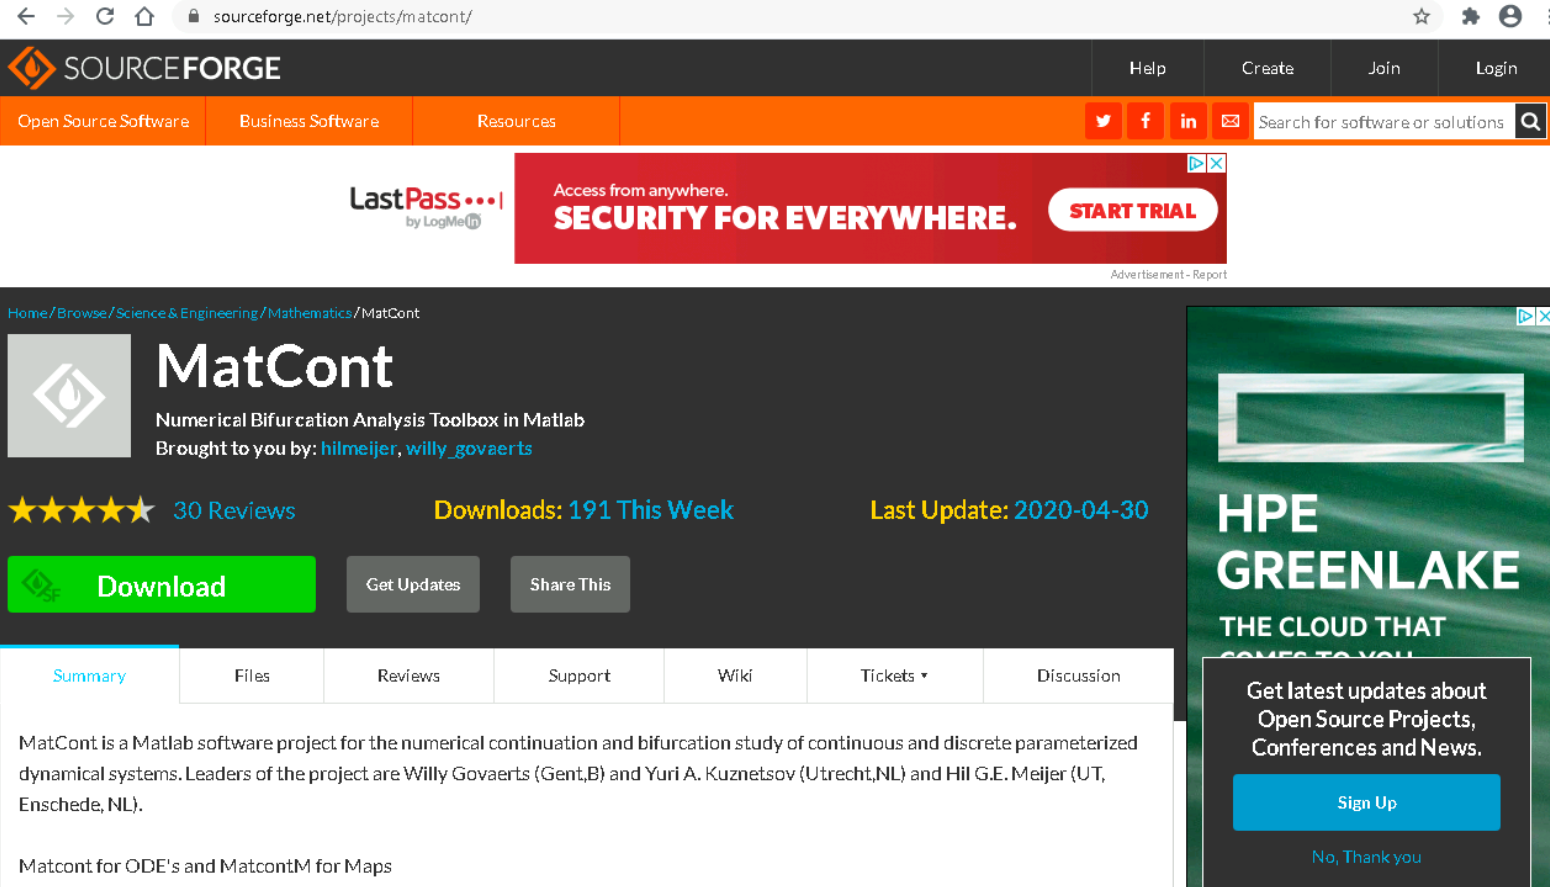
\includegraphics[width=.9\linewidth]{./MATCONT_site.png}
\end{center}

Step 1: navigate to \url{https://sourceforge.net/projects/matcont/}
\end{frame}

\begin{frame}[label={sec:orgd1ff3d8},plain]{Obtaining MATCONT}
\begin{center}
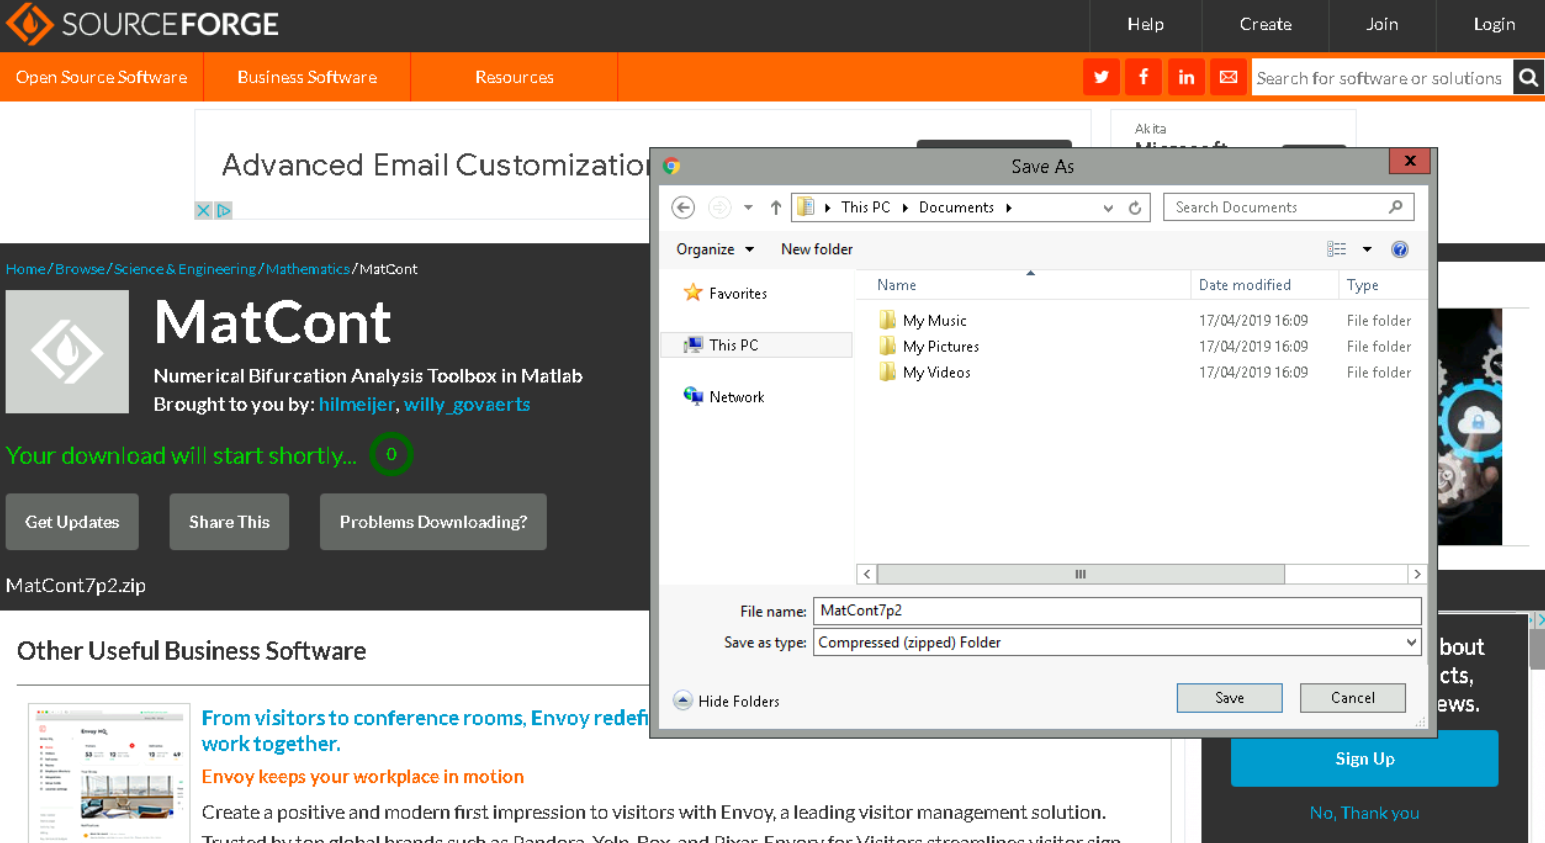
\includegraphics[width=.9\linewidth]{./MATCONT_download.png}
\end{center}

Step 2: hit the download button and save somewhere memorable
\end{frame}

\begin{frame}[label={sec:org176d356},plain]{Obtaining MATCONT}
\begin{center}
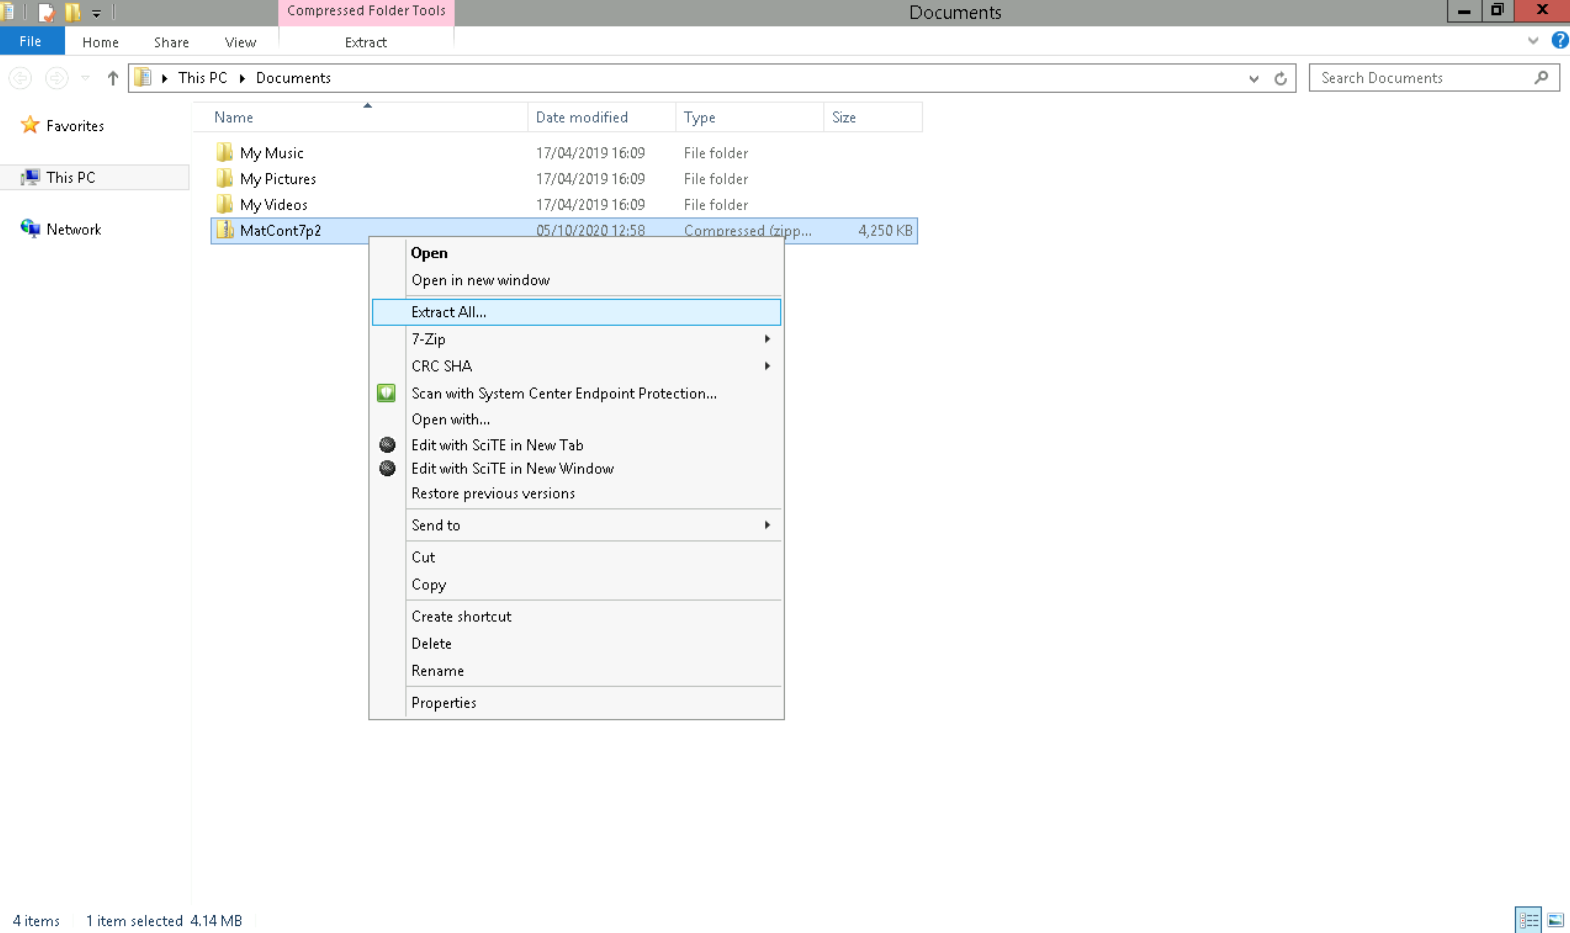
\includegraphics[width=.9\linewidth]{./MATCONT_extract.png}
\end{center}

Step 3: navigate to and extract the ZIP folder
\end{frame}
\begin{frame}[label={sec:org2fe90ce},plain]{Obtaining MATCONT}
\begin{center}
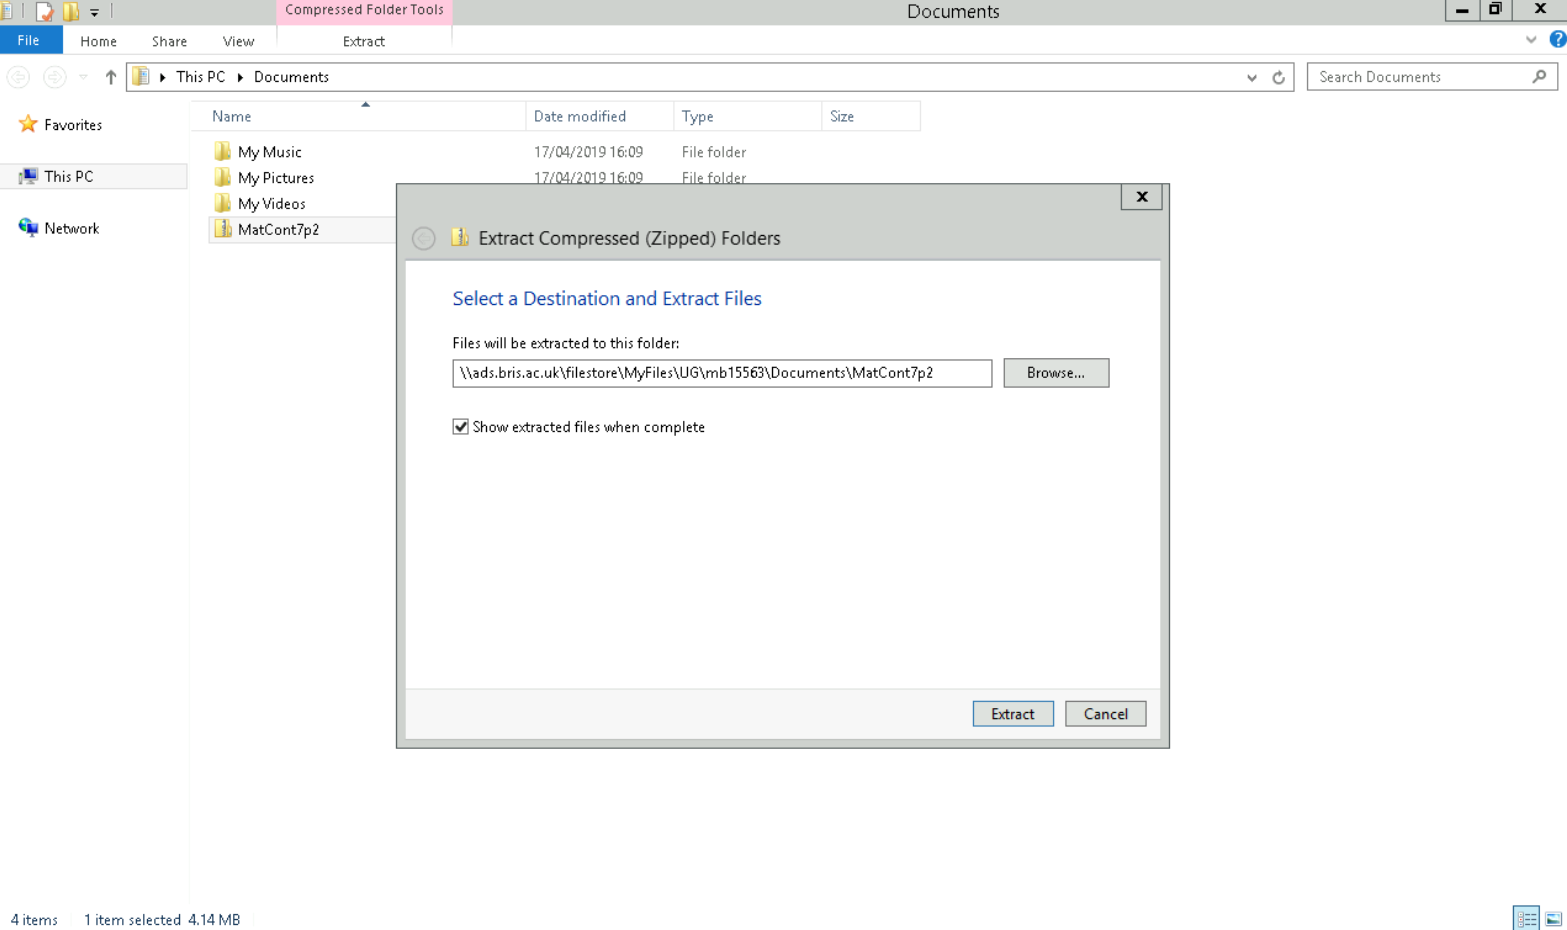
\includegraphics[width=.9\linewidth]{./MATCONT_extract2.png}
\end{center}

Step 3: navigate to and extract the ZIP folder
\end{frame}

\begin{frame}[label={sec:org2e03c17},plain]{Obtaining MATCONT}
\begin{center}
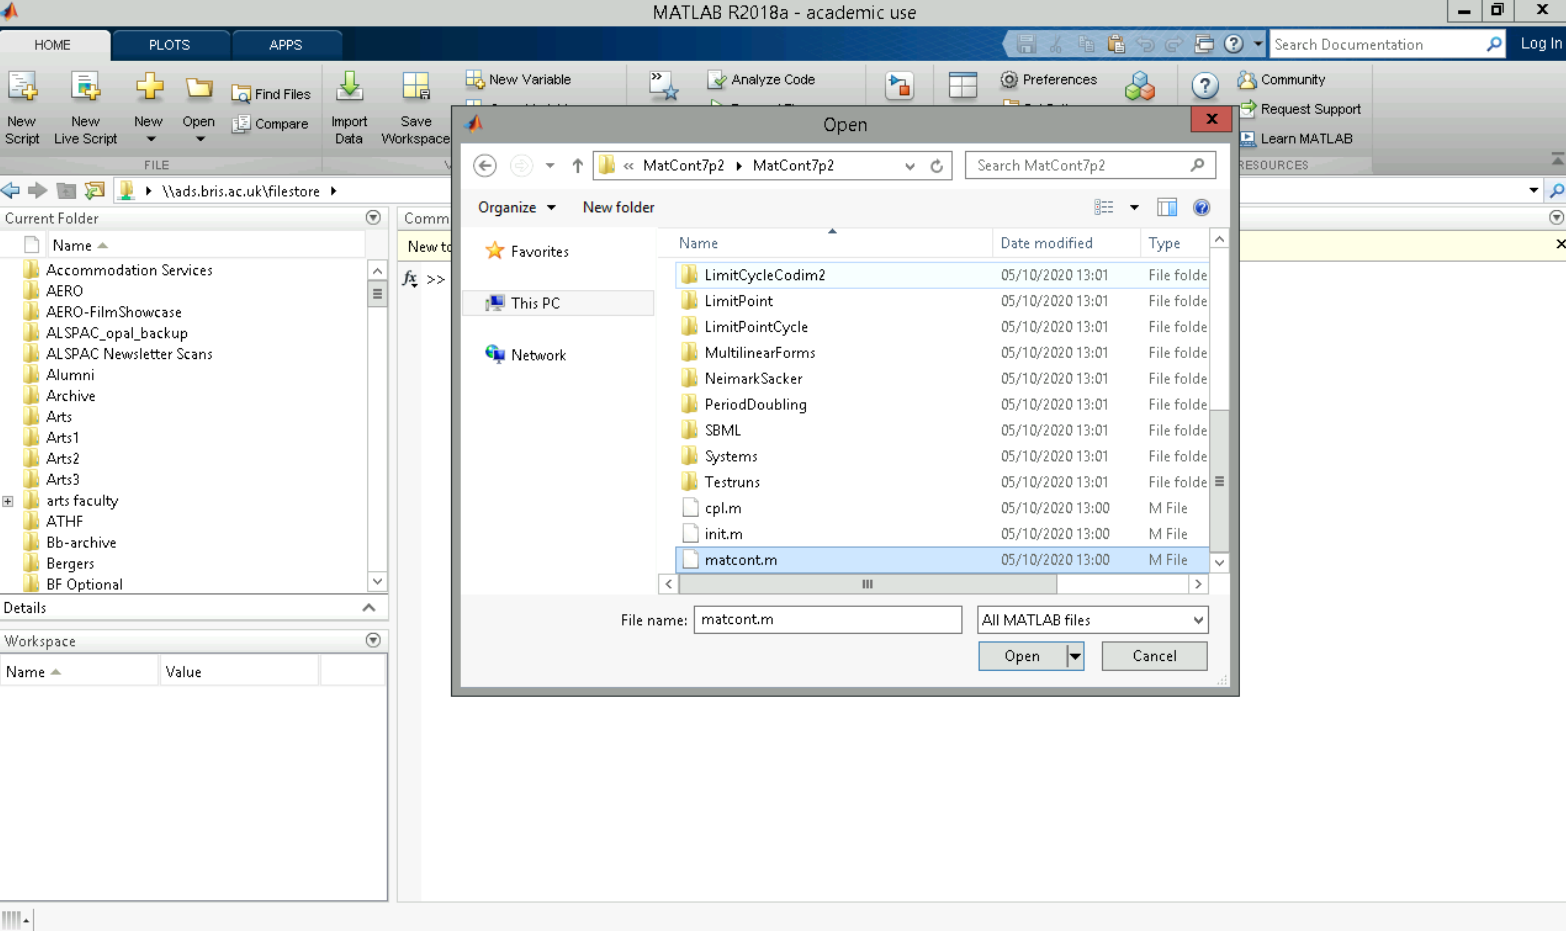
\includegraphics[width=.9\linewidth]{./MATCONT_open.png}
\end{center}

Step 4: open MATLAB and matcont.m
\end{frame}

\begin{frame}[label={sec:orge8bb3e2},plain]{Obtaining MATCONT}
\begin{center}
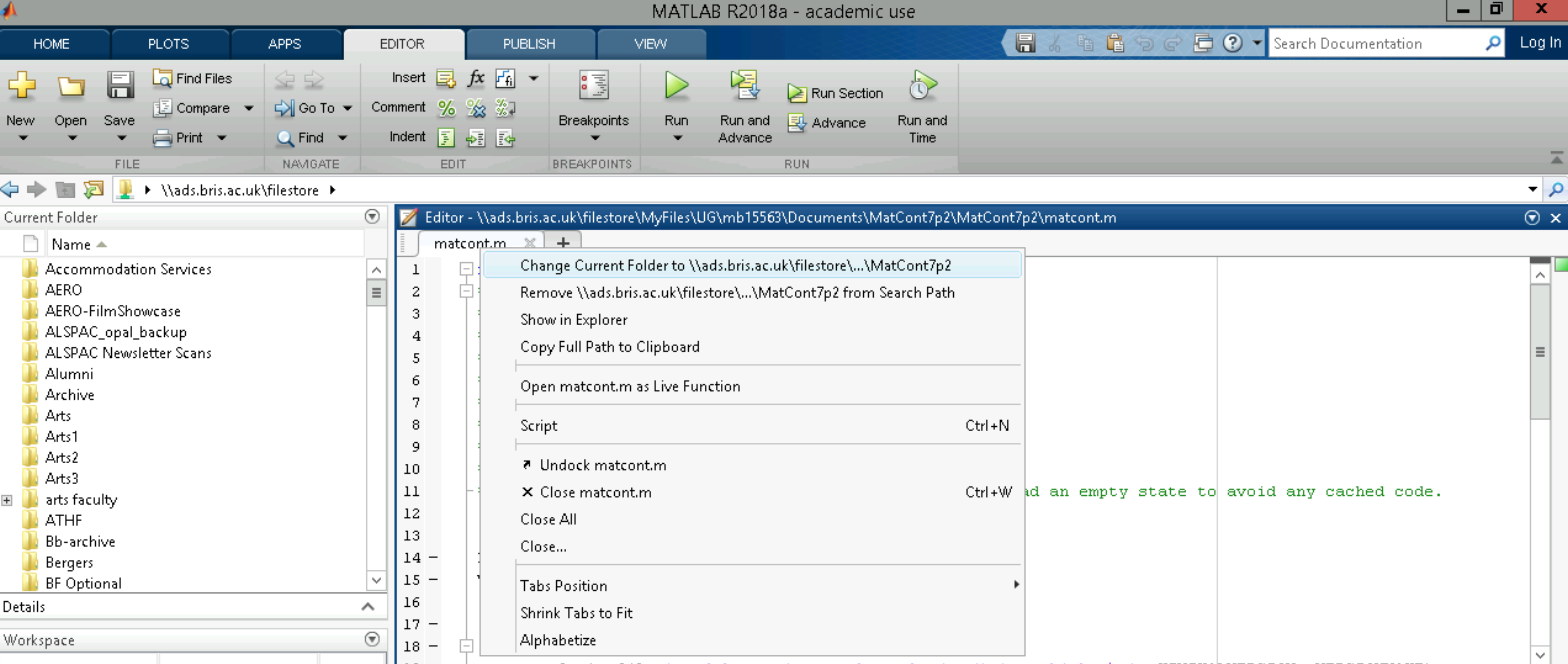
\includegraphics[width=.9\linewidth]{./MATCONT_cd.png}
\end{center}

Step 5: right-click, change current folder to \ldots{}Matcont
\end{frame}

\begin{frame}[label={sec:org1fce317},plain]{Obtaining MATCONT}
\begin{center}
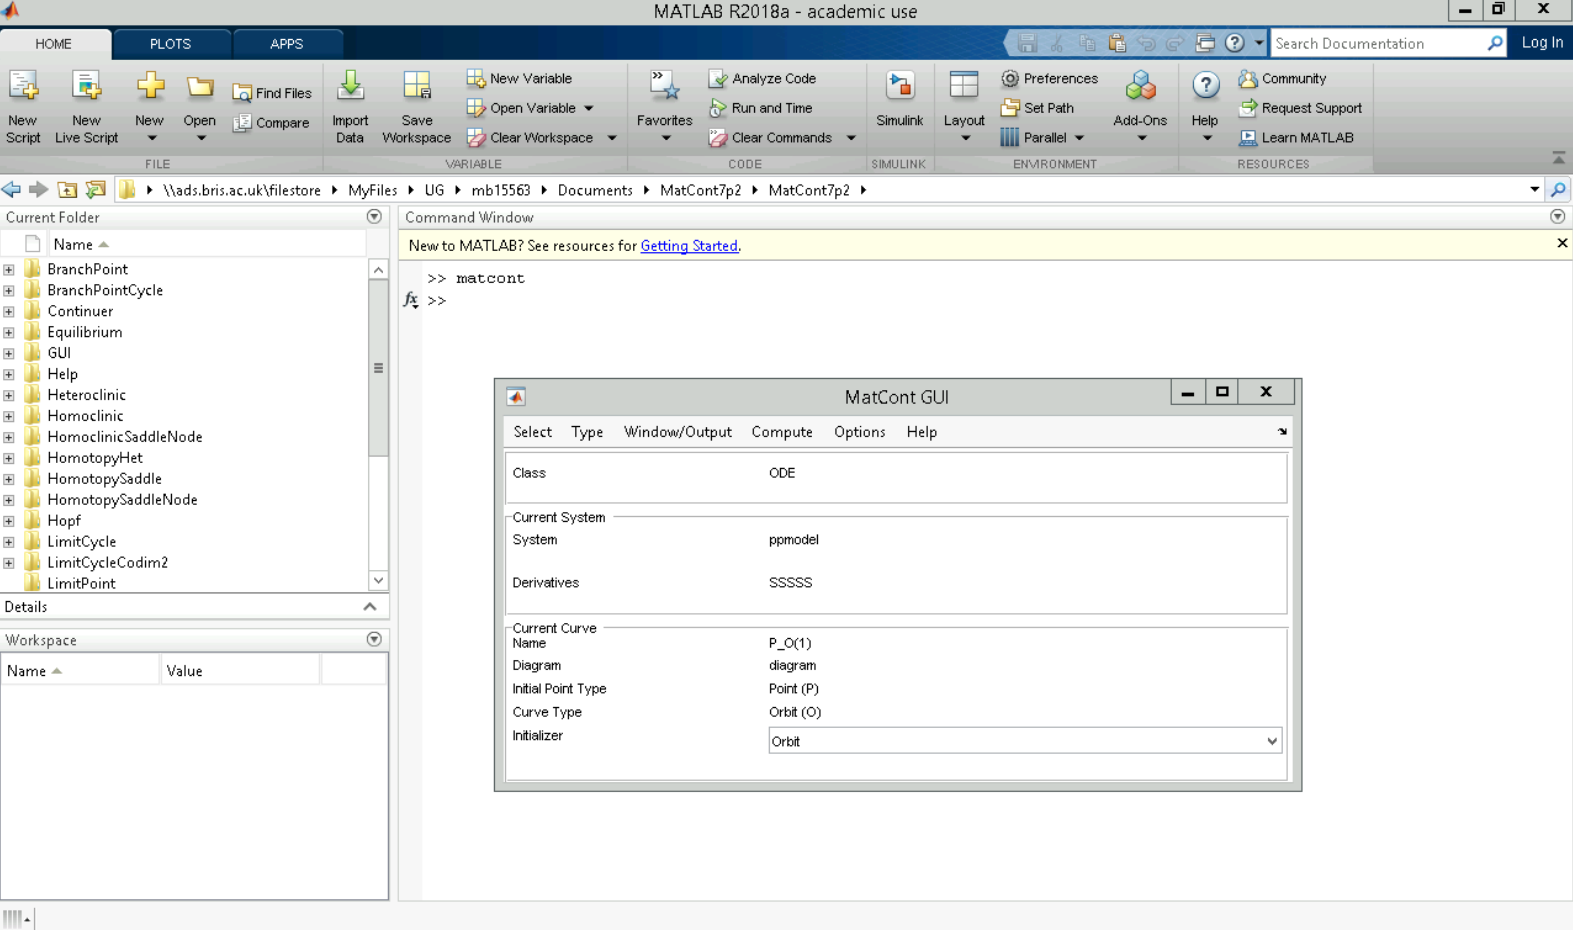
\includegraphics[width=.9\linewidth]{./MATCONT_launch.png}
\end{center}

Step 6: launch MATCONT by typing `matcont' into the prompt
\end{frame}

\begin{frame}[label={sec:orge9f3e7a}]{Issues}
MATCONT requires a compiler. If you can't run it, it'll likely be a compiler issue. The solution depends on your system. Google is your friend here.
\end{frame}

\begin{frame}[label={sec:org996a083},plain]{}
\begin{center}
live demo
\end{center}
\end{frame}

\begin{frame}[label={sec:org1f1c0bb}]{PyDSTool}
\begin{itemize}
\item Python-based continuation package
\item Simulation and analysis routines for nonlinear dynamical systems
\item More scope to integrate into scientific computing applications
\item Steeper learning curve
\item Developed by a Bristol alumnus!
\end{itemize}
\vfill    
\url{https://github.com/robclewley/pydstool}
\end{frame}
\end{document}
